\documentclass[11pt,a4paper]{article}

\usepackage[ngerman]{babel}
\usepackage[TS1,T1]{fontenc}
\usepackage[utf8x]{inputenc}
\usepackage{theorem}
\usepackage[scaled=0.9]{helvet}
\usepackage{amsmath}
\usepackage{amssymb}
\usepackage[T1]{fontenc}
\usepackage{hyperref}
\usepackage{stmaryrd}
\usepackage{pgf,tikz}
\usepackage{relsize}
\usepackage{enumitem}
\usepackage{graphicx}
\usepackage{upquote}
\usepackage{algpseudocode,amsmath,xifthen}

\newcounter{numb}
\theoremstyle{break}
\theorembodyfont{\upshape}
   	\newtheorem{aufgabe}{Aufgabe}[numb]
\setcounter{numb}{8}
\setlength{\oddsidemargin}{0cm}
\setlength{\textwidth}{16cm}
\setlength{\textheight}{23cm}
\setlength{\topmargin}{-2cm}

\usetikzlibrary{shapes,arrows,automata,positioning,decorations.fractals}
\renewcommand\familydefault{\sfdefault}


\begin{document}

\begin{minipage}[b]{\textwidth}
\parbox[t]{5cm}{%

\includegraphics[width=4cm]{unilogo}
\hfill
}
\parbox[b]{11cm}{%
%\scshape%
Heinrich-Heine-Universit\"at D\"usseldorf\\
Institut f\"ur Informatik\\
Lehrstuhl Softwaretechnik und Programmiersprachen\\
%Professor Dr.\ M.\ Leuschel
Philipp K\"orner
}

%%date
%\hfill 1.\@ August 2017\rule{0mm}{6mm}\quad\ %% <--
\end{minipage}
\begin{center}
\bf
Funktionale Programmierung -- WS 2020 / 2021\\
Reading Guide 8: Macros
\end{center}

\pagestyle{empty}

\paragraph{Zeitliche Orientierung:} Diese Lerneinheit sollte bis zum 21.01.2021 abgeschlossen werden.
%\paragraph{Abgabe des Lerntagebuchs} \"uber das ILIAS bis zum 16.5.2020 mit unbegrenzt Material, Nachfrist bis zum 23.5.2020 mit zwei Seiten A4.

\section{Material} 

\begin{itemize}
    \item 11\_macros.clj
    \item 17\_homoiconicity.clj
\item Clojure for the Brave and True, Kapitel 8
\item Clojure Reference: Macros \url{https://clojure.org/reference/macros}
\item Clojure Reference: Reader (Macro Characters) \url{https://clojure.org/reference/reader#macrochars}
\end{itemize}


\section{Lernziele}

Nach dem Bearbeiten dieser Lerneinheit sollten Sie in der Lage sein

\begin{itemize}
    \item die Auswertung von Ausdr\"ucken in Clojure vollst\"andig zu beschreiben.
    \item Homoikonizit\"at zu definieren und zu identifizieren.
    \item die Werte, die vom Reader erzeugt werden, zu benennen.
    \item Readermacros korrekt zu lesen und zu verwenden.
    \item Macros selbst zu schreiben.
    \item unhygienische Macros zu identifizieren und in hygienische Macros umzuschreiben.
\end{itemize}

\section{Highlights}

\begin{itemize}
    \item Macroexpension
    \item vollst\"andige Auswertungsregeln
    \item Helfer: \verb|macroexpand|, \verb|macroexpand-1|, \verb|macroexpand-all|
    \item Macro: \verb|defmacro|
    \item Reader Syntax: \verb|`| (Syntax-Quote), \verb|'| (Quote), \verb|~| (Unquote), \verb|~@| (Unquote-Splicing), \verb|#| (Gensym)
\end{itemize}



\section{Aufgaben}

\begin{aufgabe}[Macro]
\begin{enumerate}[label=\alph*)]
\item
Schreiben Sie ein Macro, das einen einfachen Taschenrechner mit Infix-Notation implementiert. Das erste Argument soll ein Vektor mit Bindings von Variablen auf Werte sein. Es brauchen keine Klammern und Operatorpr"azedenzen beachtet werden. Das Macro soll folgendermassen funktionieren:
\begin{verbatim}
user=> (calc [a 3] 3 + 5 * a)
24
user=> (calc [b 5 a 3] a * b + 3)
18
\end{verbatim}
\item Warum kann man den Taschenrechner nicht als Funktion schreiben?
\end{enumerate}
\end{aufgabe}

\begin{aufgabe}[DFA]
Es soll eine einfache DSL f"ur DFAs entwickelt werden.
Als Beispiel soll der Automat dienen, der Bin"arzahlen erkennt, die durch f"unf teilbar sind.
In dem Automat sind die Zust"ande entsprechend der Restklasse modulo 5 beschriftet,
also z0 sind alle Zahlen, die durch 5 teilbar sind, z3 alle Zahlen, deren Rest 3 ist, etc.

\begin{minipage}{.4\textwidth}
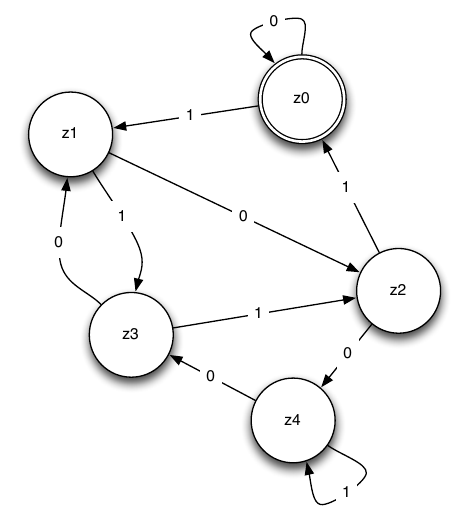
\includegraphics[scale=0.5]{dfa.png} 
\end{minipage}%
\begin{minipage}{.6\textwidth}
Die DSL soll folgendermassen aussehen:

\begin{verbatim}
(declare z0 z1 z2 z3 z4)
(def z0 (dfa-state :accept {\0 z0 \1 z1}))
(def z1 (dfa-state :reject {\0 z2 \1 z3}))
(def z2 (dfa-state :reject {\0 z4 \1 z0}))
(def z3 (dfa-state :reject {\0 z1 \1 z2}))
(def z4 (dfa-state :reject {\0 z3 \1 z4}))
\end{verbatim}

\verb|(dfa-state ... )| soll eine Funktion liefern,
die einen String bestehend aus 0 und 1 als Parameter bekommt und :accept liefert,
wenn der String ausgehend von diesem Knoten in einem akzeptierenden Zustand resultiert.
Ansonsten soll :reject zur"uckgegeben werden. 
\end{minipage}

Als Einstiegspunkt soll eine Funktion \verb|(dfa-match init text)| dienen, die ausgehend von dem Zustand init die Eingabe text verarbeitet.

\begin{verbatim}
user=> (dfa-match z0 "")
:accept
user=> (dfa-match z0 "010100010")
:reject
user=> (dfa-match z0 "0101000101")
:accept
\end{verbatim}


Testen Sie Ihre Implementierung auch einmal mit etwas l\"angeren Eingaben.

Anmerkung: Es ist wahrscheinlich, dass die erste Implementierung nicht funktioniert.
Lassen Sie sich davon nicht entmutigen und versuchen Sie, das Problem zu lokalisieren,
um es anschlie\ss{}end zu reparieren.

\end{aufgabe}


\section*{Fragen}
Bei Fragen wenden Sie sich bitte an Philipp K"orner (\texttt{p.koerner@hhu.de}).
\end{document}

